\documentclass{article}
\usepackage{graphicx} 
\usepackage{subfigure} 
\usepackage{natbib}

\usepackage{algorithm}
\usepackage{algorithmic}

\usepackage{amsthm}
\usepackage{amsfonts}
\usepackage{amssymb}
\newtheorem{mydef}{Definition}

\usepackage{listings}
\usepackage{color}

\definecolor{dkgreen}{rgb}{0,0.6,0}
\definecolor{gray}{rgb}{0.5,0.5,0.5}
\definecolor{mauve}{rgb}{0.58,0,0.82}

\lstset{frame=tb,
  language=Python,
  aboveskip=3mm,
  belowskip=3mm,
  showstringspaces=false,
  columns=flexible,
  basicstyle={\small\ttfamily},
  numbers=none,
  numberstyle=\tiny\color{gray},
  keywordstyle=\color{blue},
  commentstyle=\color{dkgreen},
  stringstyle=\color{mauve},
  breaklines=true,
  breakatwhitespace=true
  tabsize=3
}

\usepackage{hyperref}

\usepackage{amsmath}

\newcommand{\theHalgorithm}{\arabic{algorithm}}
\usepackage{icml2013} 
\icmltitlerunning{Submission and Formatting Instructions for ICML 2013}

\begin{document} 
\twocolumn[
\icmltitle{Deep Q Network\\ 
           an Approach for Guided Policy Control}
\icmlauthor{Yuan Gao}{yuan.x.gao@helsinki.fi}
\icmladdress{Department of Computer Science,
            P.O. Box 68 (Gustaf Hällströmin katu 2b) FI-00014 UNIVERSITY OF HELSINKI FINLAND}
% You may provide any keywords that you 
% find helpful for describing your paper; these are used to populate 
% the "keywords" metadata in the PDF but will not be shown in the document
\icmlkeywords{Deep Learning, Q Learning, Atari Game}
\vskip 0.3in
]
\begin{abstract} 
In this paper, We consider the methodology of the controlling agent through observing the environment of a game. With a concrete example, this paper addresses the issue of linking observed state of environment and simulated agent to perform a learning task. The algorithm that we applied in this paper is called Deep Q Network(DQN). This is the current state-of-art algorithm for a game learning agent. By comparing with the other algorithms, we are able to point out the how the algorithm outperforms the other algorithms for the same task.
\end{abstract} 
\section*{Introduction}
Reinforcement Learning(RL) algorithm has been vary successful in the many applications including robotics \cite{kober2012reinforcement}, clinical trial \cite{kuleshov2010algorithms} etc. However, when it is applied to agent control, general framework of RL suffers the curse of dimensionality. When the spaces of perception and control both become continuous, it is very hard to discretize the space porperly. Even if we can discretize the spaces, it is still very hard to find a way of performing efficient policy gradient algorithms for large amount of states. 

Similar to image classification tasks, a game control algorithm also need to observe and process images. In recent years, one algorithm called Convolutional Neuro Network(CNN) has been suggested\cite{lecun1998gradient}. The CNN is a multi-layer neuro netowrk with one input layer, several hidden layers and output layers. As it can detect the features of the graph automatically, it has been treated as a very important preprocessing step for agent control algorithms.

The combination of value function-based RL and CNN can be considered as relatively efficient agent control algorithm. On one hand, as stated before, the RL algorithm provides the entire analysis framework including mathematical modelling and optimization techniques. On another hand, the CNN reduces the dimensions of input images. 

The organization pf this paper is as follows. We first introduce the problem that we would like to solve. After that we take previuous lines of analysis one step further in Section 2 and 3 by introducing value-function-based RL and CNN which forms the foundation of our algorithm. In Section 4, we will cobine these methods and introduce the algorithm Deep Q Network(DQN)for our problem. Results are shown in Section 5. We gathered some statistics for performance of this algorithm. Conclutions are drawn in Section 6. 

\section{Problem Definition}
We would like to develop an AI agent that can play Atari games automaticly.

The Atari video games was release in year 1977. Selling for 30 millions consoles, Atari games are considered fun and successful. Now the Atari games are not considered as commercial products, a reinforcement learning platform Atari Learning Environment(ALE) is established for the research in order to ease the engineering difficulty of the research\cite{bellemare12arcade}. There are several reasons of applying this environment. First of all, the environment provides several standard actions for the agent. Simultaneously, the game offers the researcher to compare their work easily. Finally, the state of Atari game is relatively easy to be observed and analysed. The frame is just a 160*210 matrix and its RAM is only 128 bytes. It is simple enough for modern computer with high-frequency CPU to deal with.

The Arcade Learning Environment provides an object-oriented framework for testing different agent on different games. The Figure~\ref{atari_game} shows several games supported by the ALE.
\begin{figure}[h!]
\centering
{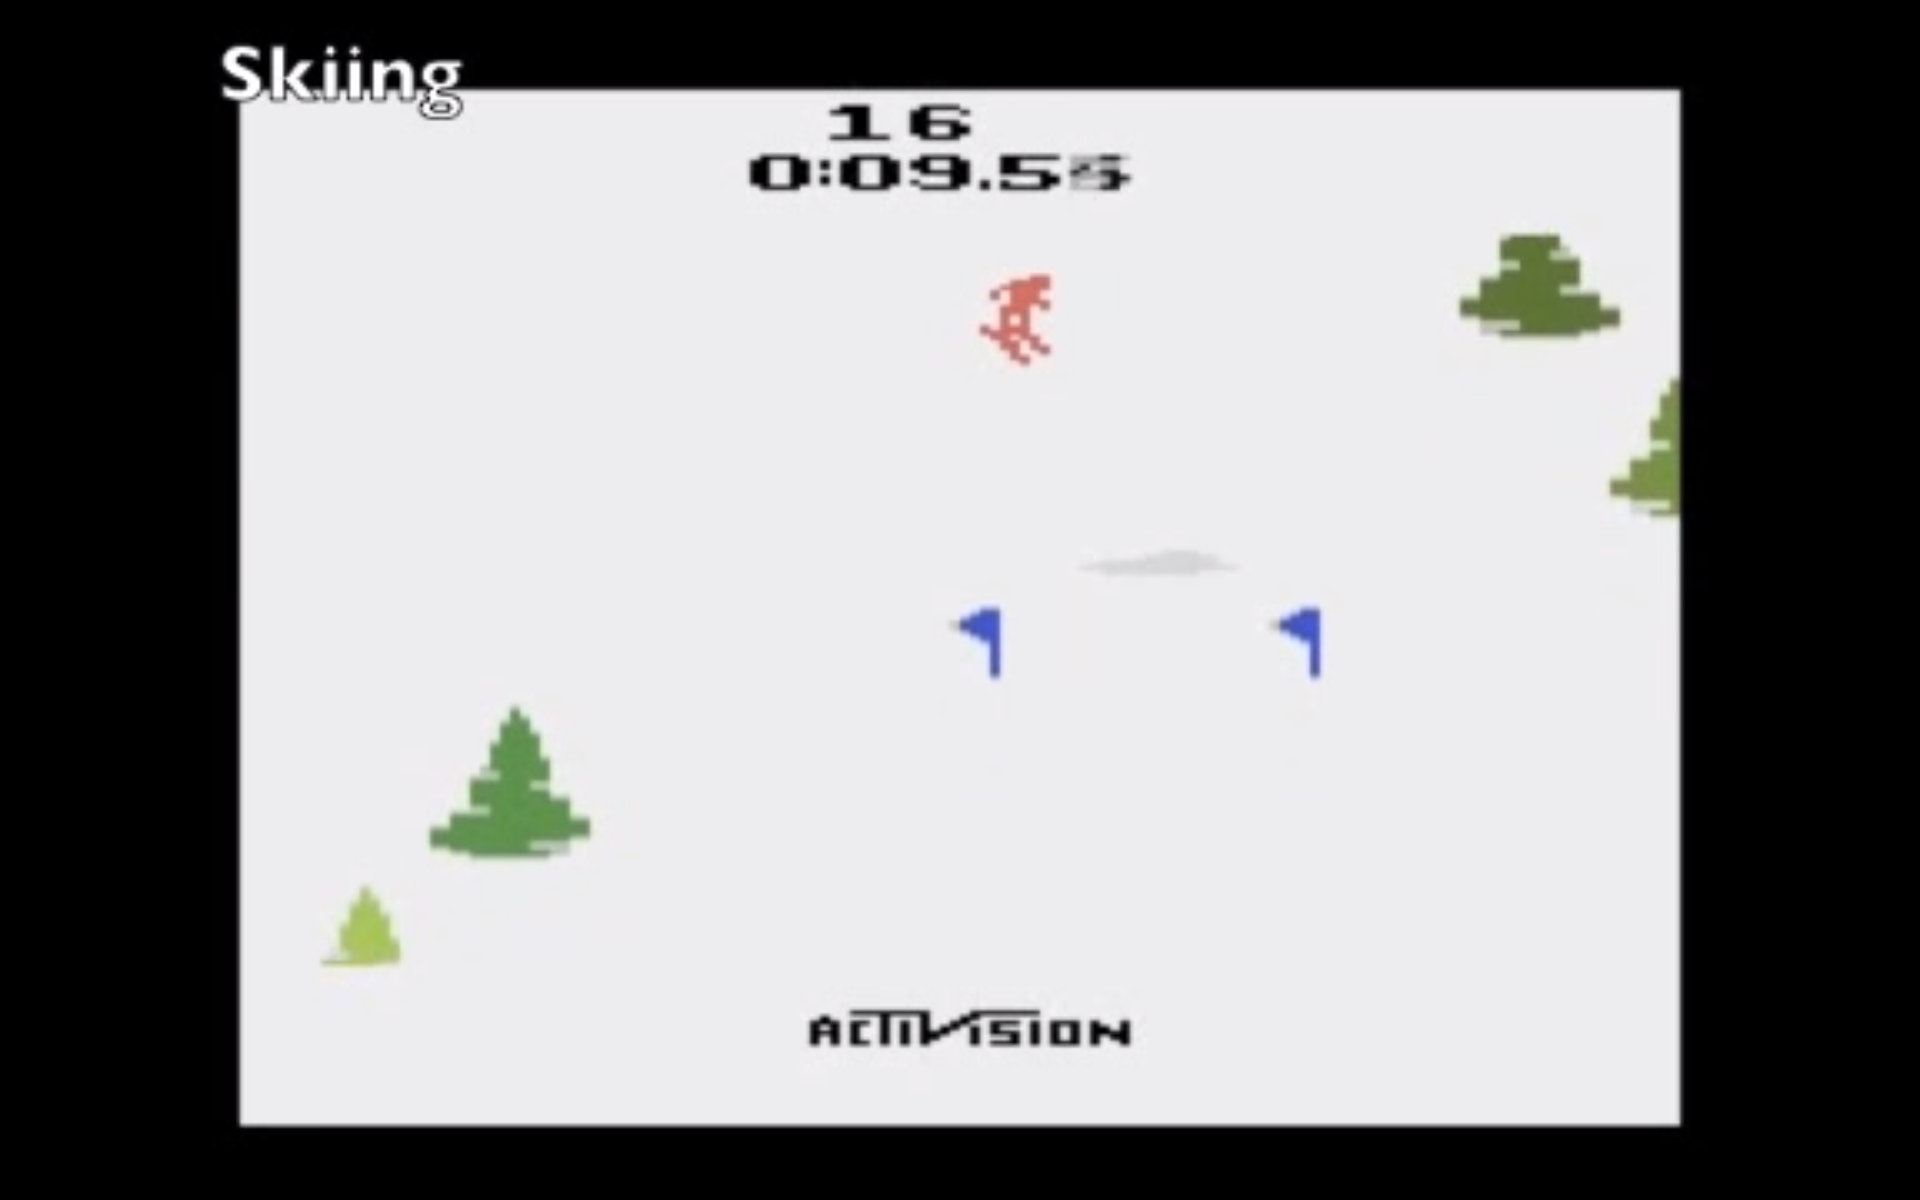
\includegraphics[width = 0.23\textwidth]{1}} 
{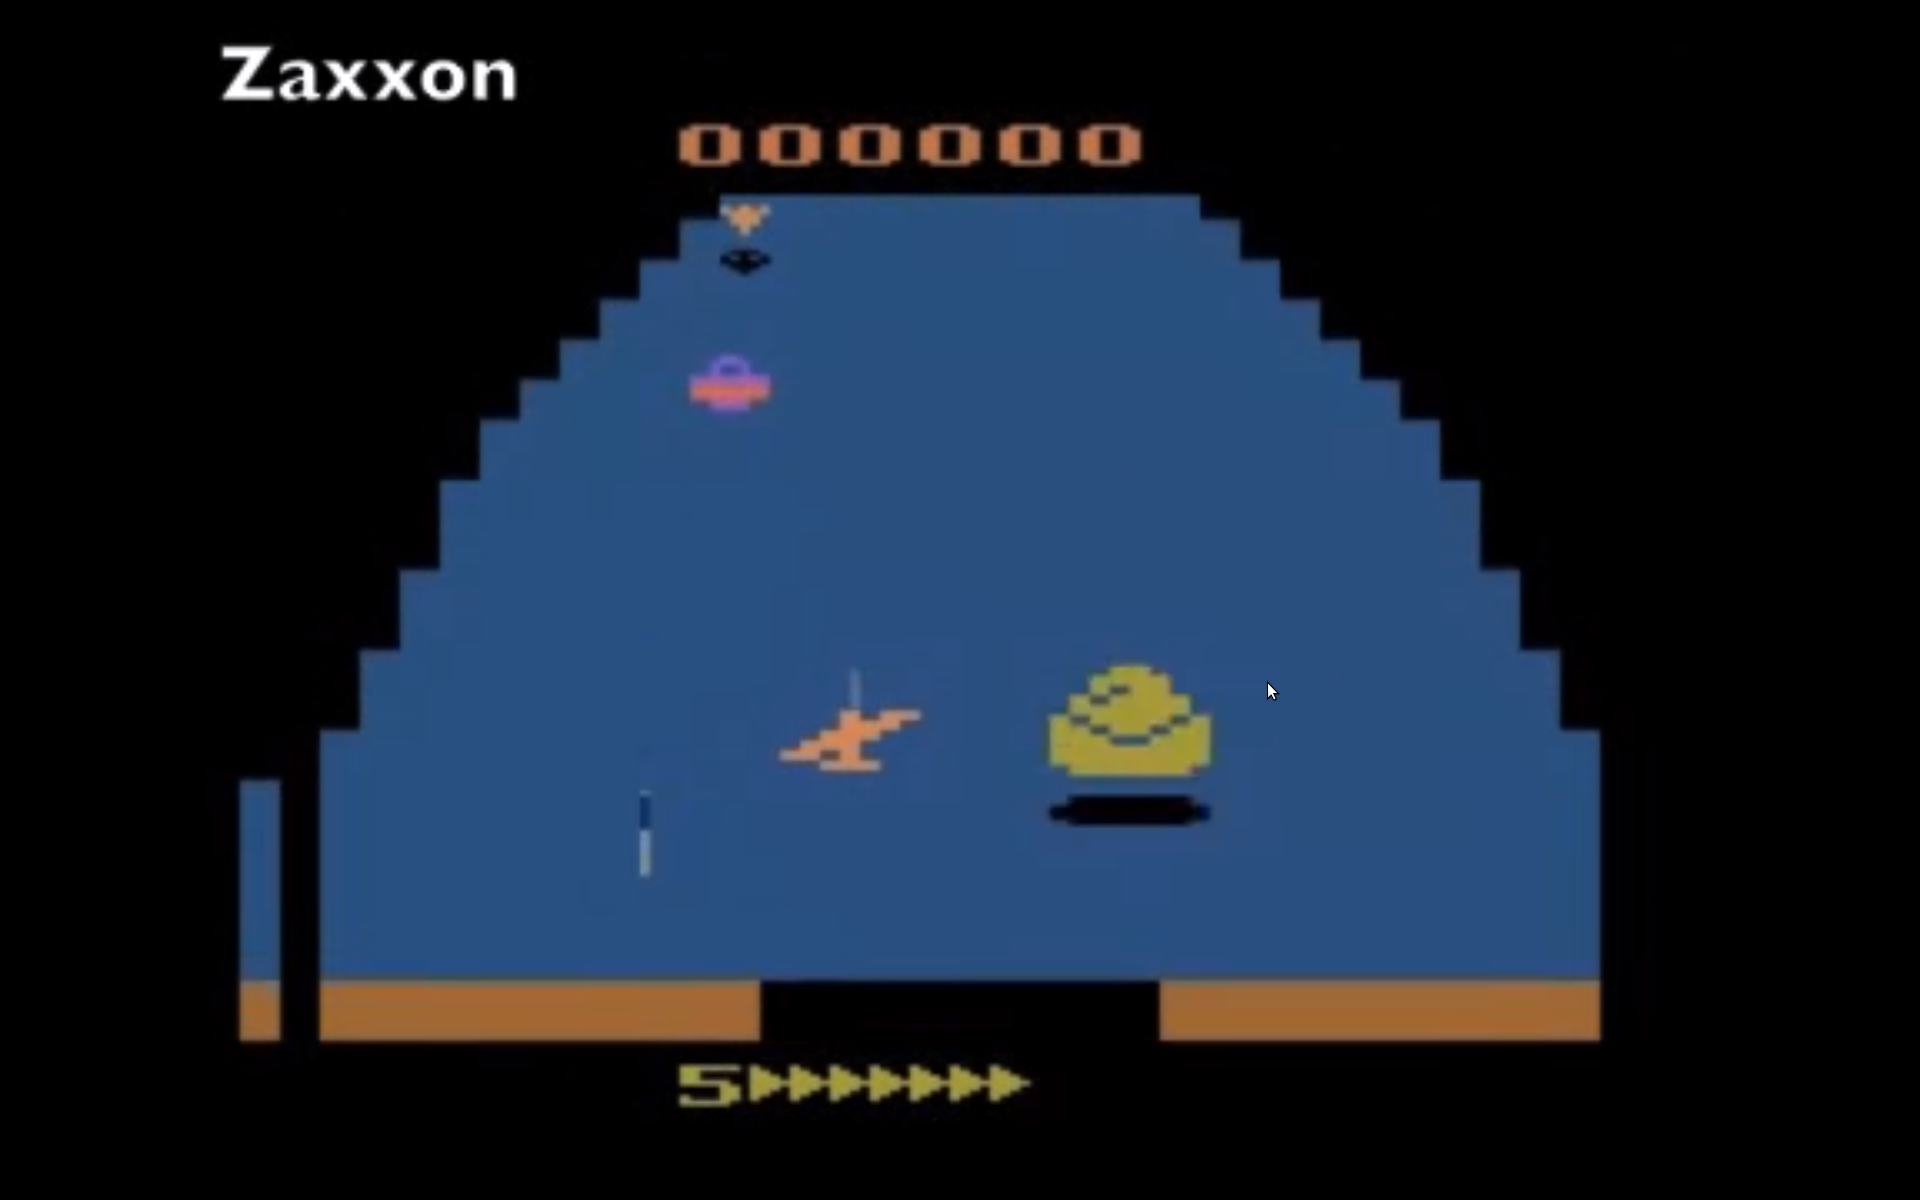
\includegraphics[width = 0.23\textwidth]{2}}\\
{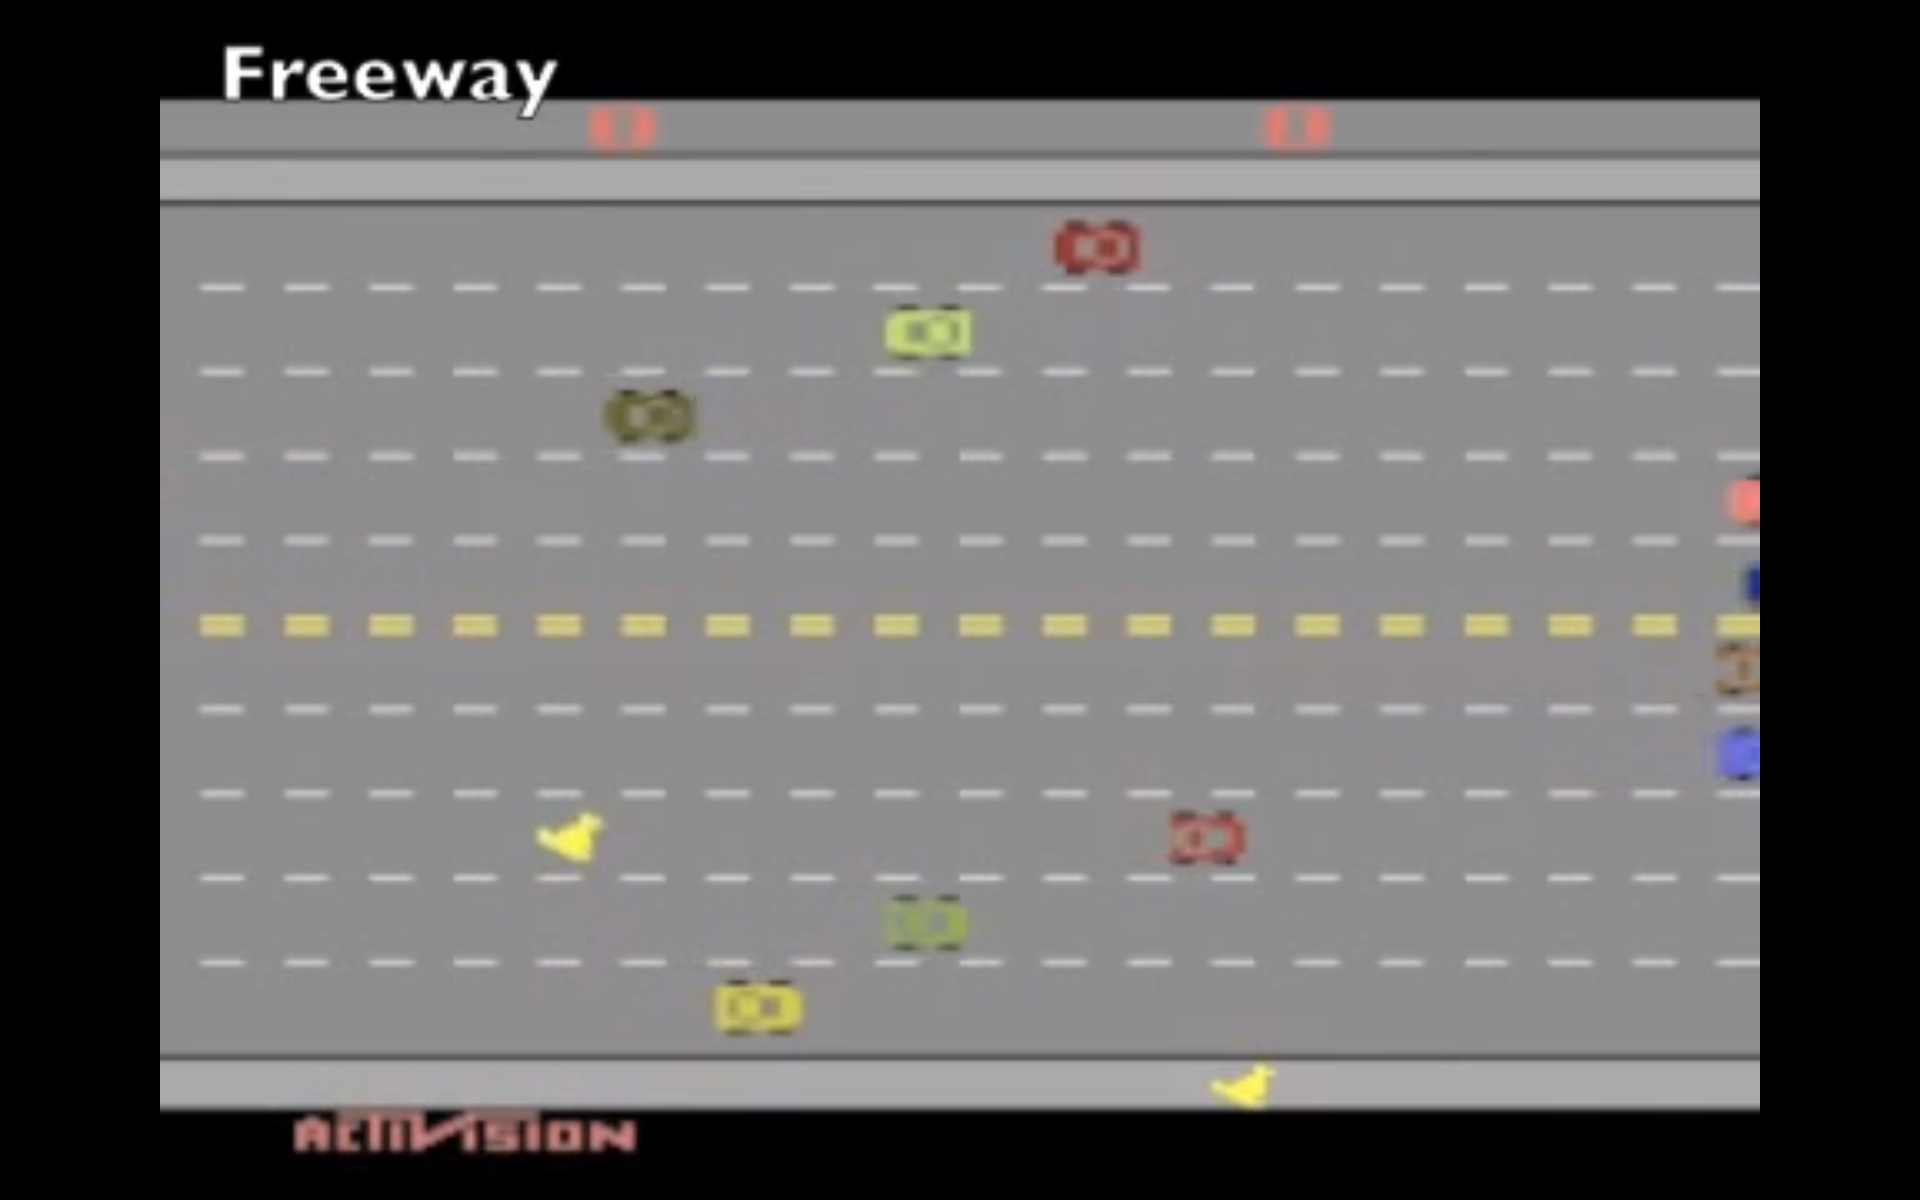
\includegraphics[width = 0.23\textwidth]{3}}
{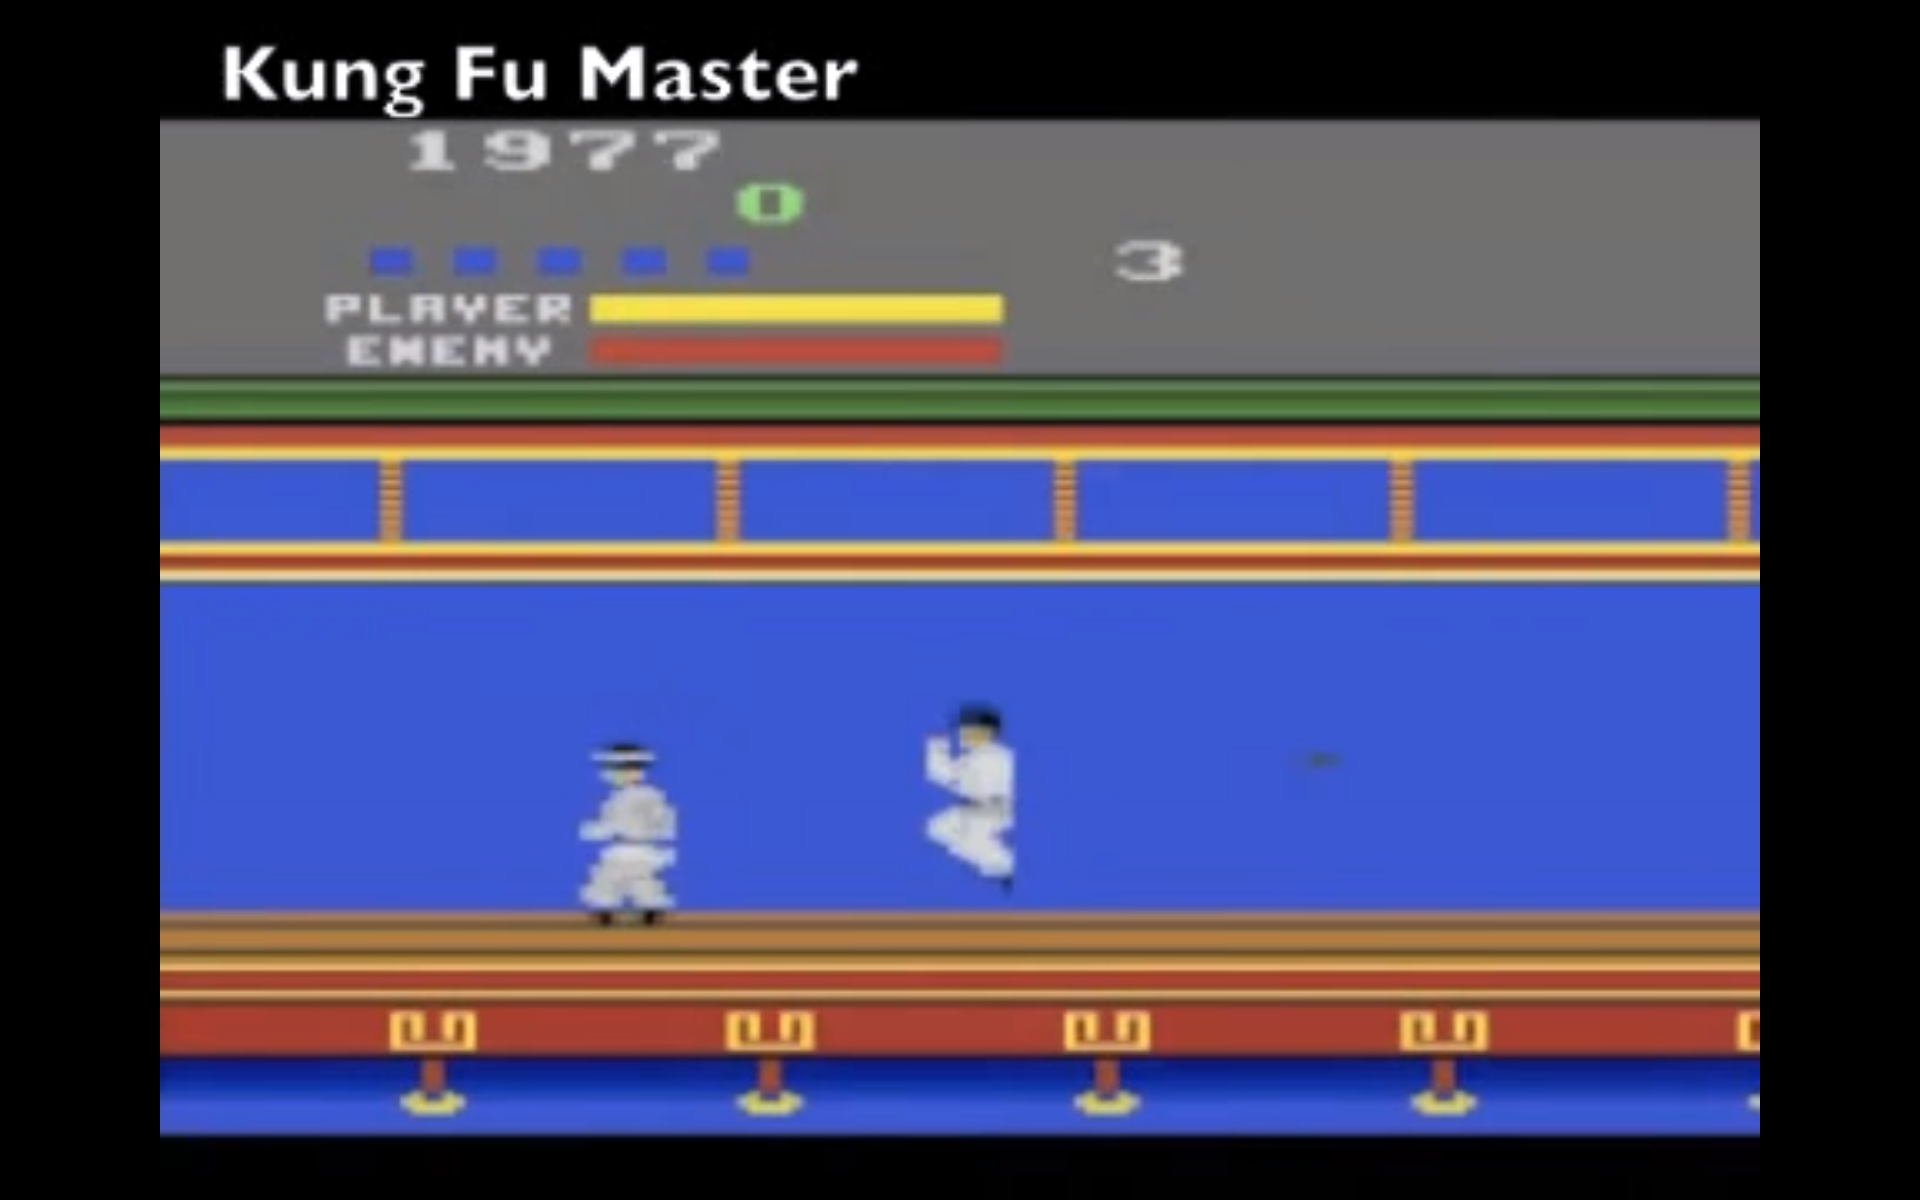
\includegraphics[width = 0.23\textwidth]{4}} 
\caption{This figure shows the basic games of the Atari Learning Environment(ALE) of reinforcement learning research. On the top left corner is famous atari 2600 game Skiing. The top right corner is Zaxxon. The down left corner is Freeway. The down right corner is KongFu Mater. These games are representatives of the testing environment.}\label{atari_game}
\end{figure}

For achieving a goal of controlling an agent, we have consider two things - observation and control. 

The trandistional feature extraction algorithm from a game image includes Basic Abstraction of the ScreenShots (BASS), 	Detecting Instances of Classes of Obsjects(DISCO) and Console Memory Reading \citep{naddaf2010game}. The newly advanced unsupervised feature detection method in image classification is CNN.

The original CNN(Figure~\ref{cnn}) is a feed forword nuero networks meant to deal with the image classification problem. It has become the state-of-art algorithm in this field. These kinds of network always involve an input layer, even hidden layers, a fully connected output layer. The hidden layers consist several times of combination of two processes. First of them is convolutional layer and second of them is downsampling layer.

The convolutional layer uses several convolutional kernels(filters) to convolve through the image, after which downsampling layer reduces the size of image to be processed.

After processing like this for several layers, the cnn than use a full layer to classify them.

In our project, we modify network to output instead of classification labels, we output corresponding actions in the network.

\begin{figure*}
\centering
{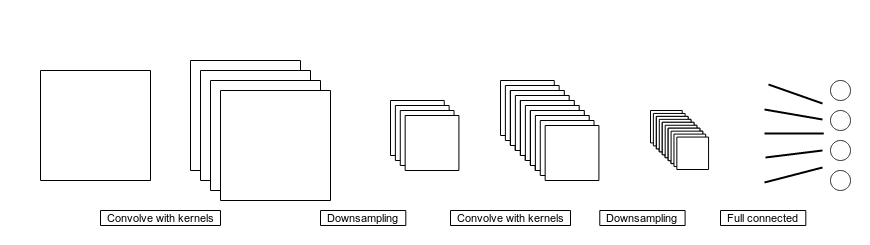
\includegraphics[width = 1\textwidth]{cnn}} 
\caption{This figure shows the structure of CNN, specifically LeNet-5 named after Yang LeCun. This CNN contains five layers of nuero network including two covolutional layers, two downsampling layers, one full connected layer. Along with the procedure in this figure, at first the image locally convolves with, normally, a 5x5 sliding matrix filter and generate several feature maps. After the convolution, we use some way to downsample the image. Normally some non-linear machanism(MaxPooling) is used. The previous step ensures the important features are observed by the algorithm. As long as we getting enough samples, a full layer is then applied to classify them into lables.}\label{cnn}
\end{figure*}

\subsection{Interact With Environment}

ALE provides a framework of interacting with enviroment. Apperently, at least the game status are parameters describing the game. The status are also the the status of the games.

For previous defined CNN, we still need preprocess the image. In our project, we use the four stacked frames to be the one input of CNN. We discribe this process by a function $\varphi(\cdot)$. Function $\varphi(\cdot)$ is defined to take four 160x210 pixels image as an arguement and output the four grayed 100x100 images.

Without loss of generality we define a tuple 

$$e_t = (s_t, a_t, r_t, s_{t+1})$$ to be one-time experience of the agent where $s_t$ is returned value by the function $\varphi(\cdot)$, $a_t$ is the action at time $t$, $r_t$ is the instant reward at time $t$.  

Then we define a set $\mathcal{D} = \{e_1, e_2, e_3, \cdots\}$ to be maintained in each iteration as consequence, we can use minibatch stochastic gradient descent method to optimaze the parameters of the nueronetwork.

Specifically, as Figure~\ref{function_output} shows, $s_t$ is represented by the four downsampled imgage. And as we use a very classic game beakout for testing, the actions $a_t$ in this game can only to be left or right. As a consequence, the output layer for this network is set to two indicating two actions, though while gaming the game, several other actions are also needed including fire(starting game) and pause for configuration issues. $r_t$ is defined to be only corresponded to score though it can also be related to time but it belongs to the further discussion.

In the original papar, it is pointed out that they have trained the nueronetwork more than million iterations. In our project, we just iterate through the network until it can behave as it apparently learned something.
\section{Formalization of Reinforcement Learning}
In this section, we formalize the problem of the reinforcement learning for the further description of the problem. We will formalize the concepts of the Markov Decision Process, Policy and Reinforcement learning consequently.
\begin{mydef}
MDPs
A Markov Decision Process(MDP) is defined by a tuple $(\mathbb{S},\mathbb{A},T(.,.),R(.,.))$\footnote{In some definition, the initial state $s_0$ is added to the tuple.}
\end{mydef}
In the definition
\begin{itemize}
\item $\mathbb{S}$ is defined as set of states.
\item $\mathbb{A}$ is defined as set of actions.
\item $T(a,s)$ is the transition function that defines the transition distribution over all destination states. $s' = T(a,s)$.
\item $R(a,s)$ is the reward function that defines the transition distribution over all destination states. $r = R(a,s)$.
\end{itemize}
This probabilistic model is Markovian as the Markov property holds for both transition function and reward function.
\begin{mydef}
\textit{Policy}.
A Policy $\pi$ is an injection that maps state to action. $\pi:\mathbb{S}\rightarrow\mathbb{A}$
\end{mydef}
A policy is important for determining the so-call policy value. This value is used for finding the optimal policy as it is similar to a problem that try to find maximum value for all states.
\begin{mydef}
\textit{Policy Value}.
A policy value associated with a state $s \in \mathbb{S}$ is defined as a value $v_s(\pi) = V(s,\pi)$  where $v_s(\pi)  \in \mathcal{R}$. $V(s,\pi)$ represents the expected reward when the agent follows the policy $\pi$.
\end{mydef}
With a finite setting (i.e. finite states, finite actions, finite epoch $T$). $V(s,\pi)$  is defined as 
\begin{equation}
V(s,\pi) = \mathbf{E}\left[\sum_{i=0}^{T-t}\gamma^i r(s_{t+i},\pi(s_{t+i}))|s_t = s\right]
\end{equation}
Where $\gamma$ is the discount factor that ranges from 0 to 1.
\begin{mydef}
\textit{Bellman's equation}.
\begin{equation}
V(s,\pi) = \mathbf{E}\left[ R(s,\pi(s)) \right]+ \gamma \mathbf{E}\left[V(T(s,\pi(s)),\pi)\right]
\end{equation}\label{bellman}
\end{mydef}
Here we state the Bellman's equation without proof. This function determines the iterative update for the algorithm. Further information of proof can be found in Mohri's book\cite{mohri2012foundations}.

The Q-learning is an iterative algorithm that implementes Bellman's equation as in Definition~\ref{bellman}\citep{watkins1989learning}. Each iteration, the algorithm updates the expectation that algorithm can learn so far. 

\section{Deep Architecture}
In 2006, Hiton et al. published a paper \cite{hinton2006fast} to discus about why and how should we use the more-than-one hiddent layer neuronetworks to implement elegant algorithm. This so-called "deep architecture" philosophy has led to sevreal state-of-art or almost atate-of-art algorithms in artificial intelligence.  \cite{lecun1998gradient} \cite{hinton2012deep}. 

Two families of deep learning are introduced through the research and development. One of them is Deep Nuero Network \cite{fukushima1980neocognitron}\cite{lecun1998gradient}. Another one is Deep Bozlman Machine (DBM)\cite{hinton1986learning} with hidden units.

In recent years, deep learning architechtures are normally studied in supervised and unsupervised manner. Although there are some atemptations \citep{mnih2013playing}\citep{lenz2013deep}, generally deep learning frameworks are not studied in reinforcement learning. Even for these temptations, the interests are mainly on learning the image representations of system.

In our project, we implemente one of the attemps for reinforcement learning problem. This problem modifies the Convolutional Nuero Network(CNN)\cite{lecun1998gradient} to associate(learn) the feutures of environment with the actions.





\begin{figure}[h!]
\centering
{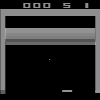
\includegraphics[width = 0.21\textwidth]{test_input_0}} 
{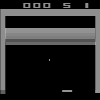
\includegraphics[width = 0.21\textwidth]{test_input_1}}\\ 
{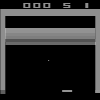
\includegraphics[width = 0.21\textwidth]{test_input_2}}
{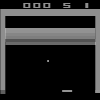
\includegraphics[width = 0.21\textwidth]{test_input_3}} 
\caption{This figure shows the input of CNN for game breakout. The function $\varphi(\cdot)$ convert the RGB(red, green, blue ) image to gray-scale image and further downsample it to four 100x100 images. The number at the top left corner shows the current score. The number at top middle shows the lives of the agent. The only moving object white dot is a ball. And the white bar in the middle is the agent that can reflect the ball to the breaks.}\label{function_output}
\end{figure}

\section{Deep Q Network}

In this section, we combine what have been mentioned above to form a concret description of DQN.

DNQ was proposed by DeepMind campany in 2013, it is the current state of art algorithm for game-playing agent. It combines concepts of nueronetwork and q-learning. The DNQ mimics the behavior in a sense that it gives an action and get a reward. Based on the reward, it optimizes the parameters and make a reasonable selection of actions next time. It also mimics the behavior of randomly selecting the a action with probability $\sigma$.

By mantaining a set $\mathcal{D}$ and uses minibatch optimazation, the network is able to gain expereiences to control the agent.

A full functional DQN consists fellowing parts.

\begin{enumerate}
\item capture four screen matrices of continuous frames.
\item stack four screen matrix into a signal vector.
\item gray-scale the screen matrix.
\item linearly downsample to a signal 4 x 100 x100 vector.
\item input 4 x 100 x100 to input layer of DQN.
\item feedforward and get output.
\item get reward and store $e_t$ into set $\mathcal{D}$.
\item randomly selects experieces from  $\mathcal{D}$.
\item backpropagate and train DNQ.
\item store the highest output and corresponding action
\item with a possibility $0 \leq \sigma \leq 1$, the algorithm excutes action randomly otherwise excutes the output action.
\item repeat from step one.
\end{enumerate}
\begin{figure}[H]
\centering
{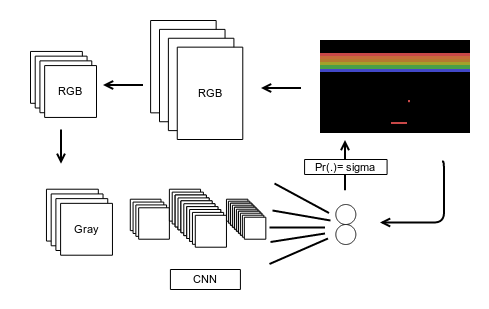
\includegraphics[width = 0.5\textwidth]{dqn}} 
\caption{This figure shows the structure of the DQN. Along with steps above, at beginning, images are preprocessed before entering the CNN and then after getting the reward,  we train the CNN with reward.}\label{dqn}
\end{figure}

There are several issues to be discussed in DNQ as there are several variations. One essential property lies in the how would downsample the image unser this senarior. 

One popular downsampling methods in CNN include the maxpolling.

% TODO
\section{Testing}

A previous stated, we mainly use the game breakout for testing. Besides using DNQ for this game, we also use an algorithm called HyperNEAT to see whether they make a distinct difference.

HyperNEAT is a generative encoding that evolves the parameters and archtectures by NeuroEvolution of Augmented Topologies (NEAT) algorithm\citep{stanley2006exploiting}. It uses a so-called Compositional pattern-producing networks (CPPNs) to complete this task. CPPN differs with current nueronetwork in which it uses different activation function. NEAT is an efficient algorithm that evolve the network efficently.

It the original paper \citep{mnih2013playing}, it is pointed out that DNQ outperforms HyperNEAT for most of the tested games.


\section{Six}
\section{Seven}
% In the unusual situation where you want a paper to appear in the
% references without citing it in the main text, use \nocite
\nocite{langley00}
\bibliography{seminar_report}
\bibliographystyle{icml2013}
\end{document} 
% This document was modified from the file originally made available by
% Pat Langley and Andrea Danyluk for ICML-2K. This version was
% created by Lise Getoor and Tobias Scheffer, it was slightly modified  
% from the 2010 version by Thorsten Joachims & Johannes Fuernkranz, 
% slightly modified from the 2009 version by Kiri Wagstaff and 
% Sam Roweis's 2008 version, which is slightly modified from 
% Prasad Tadepalli's 2007 version which is a lightly 
% changed version of the previous year's version by Andrew Moore, 
% which was in turn edited from those of Kristian Kersting and 
% Codrina Lauth. Alex Smola contributed to the algorithmic style files.  
